% !TEX TS-program = pdflatex
% !TEX encoding = UTF-8 Unicode

% This is a simple template for a LaTeX document using the "article" class.
% See "book", "report", "letter" for other types of document.

\documentclass[11pt]{article} % use larger type; default would be 10pt

\usepackage[utf8]{inputenc} % set input encoding (not needed with XeLaTeX)

\usepackage{mathtools}

\DeclarePairedDelimiter\abs{\lvert}{\rvert}%
\DeclarePairedDelimiter\norm{\lVert}{\rVert}%

% Swap the definition of \abs* and \norm*, so that \abs
% and \norm resizes the size of the brackets, and the 
% starred version does not.
\makeatletter
\let\oldabs\abs
\def\abs{\@ifstar{\oldabs}{\oldabs*}}
%
\let\oldnorm\norm
\def\norm{\@ifstar{\oldnorm}{\oldnorm*}}
\makeatother

%%% Examples of Article customizations
% These packages are optional, depending whether you want the features they provide.
% See the LaTeX Companion or other references for full information.

%%% PAGE DIMENSIONS
\usepackage{geometry} % to change the page dimensions
\geometry{a4paper} % or letterpaper (US) or a5paper or....
% \geometry{margin=2in} % for example, change the margins to 2 inches all round
% \geometry{landscape} % set up the page for landscape
%   read geometry.pdf for detailed page layout information

\usepackage{graphicx} % support the \includegraphics command and options

% \usepackage[parfill]{parskip} % Activate to begin paragraphs with an empty line rather than an indent

%%% PACKAGES
\usepackage{booktabs} % for much better looking tables
\usepackage{array} % for better arrays (eg matrices) in maths
\usepackage{paralist} % very flexible & customisable lists (eg. enumerate/itemize, etc.)
\usepackage{verbatim} % adds environment for commenting out blocks of text & for better verbatim
%\usepackage{subfig} % make it possible to include more than one captioned figure/table in a single float
\usepackage{caption}
\usepackage{subcaption}
\usepackage{breqn}

% These packages are all incorporated in the memoir class to one degree or another...

%%% HEADERS & FOOTERS
\usepackage{fancyhdr} % This should be set AFTER setting up the page geometry
\pagestyle{fancy} % options: empty , plain , fancy
\renewcommand{\headrulewidth}{0pt} % customise the layout...
\lhead{}\chead{}\rhead{}
\lfoot{}\cfoot{\thepage}\rfoot{}

%%% SECTION TITLE APPEARANCE
\usepackage{sectsty}
\allsectionsfont{\sffamily\mdseries\upshape} % (See the fntguide.pdf for font help)
% (This matches ConTeXt defaults)

%%% ToC (table of contents) APPEARANCE
\usepackage[nottoc,notlof,notlot]{tocbibind} % Put the bibliography in the ToC
\usepackage[titles,subfigure]{tocloft} % Alter the style of the Table of Contents
\renewcommand{\cftsecfont}{\rmfamily\mdseries\upshape}
\renewcommand{\cftsecpagefont}{\rmfamily\mdseries\upshape} % No bold!

%%% END Article customizations

%%% The "real" document content comes below...

\title{Trapezoid Velocity Trajectory Generator}
\author{Chien-Liang Fok}
%\date{} % Activate to display a given date or no date (if empty),
         % otherwise the current date is printed 

\begin{document}
\maketitle

\section{Introduction}

The velocity trajectory takes the shape of a trapezoid as shown in Figure~\ref{fig:velocity_vs_time}.

\begin{figure}[tbh]
    \centering
    \begin{subfigure}[b]{0.35\textwidth}
        \centering
        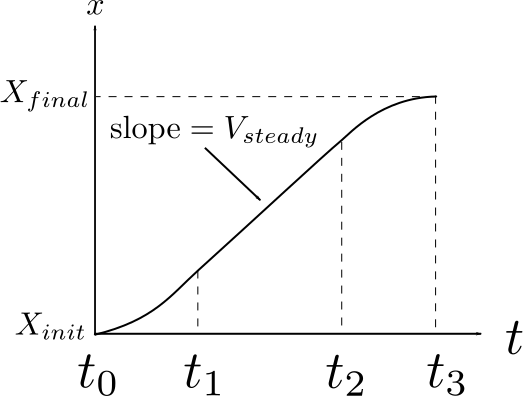
\includegraphics[width=\textwidth]{position_vs_time.png}
        \caption{Position vs. Time}
        \label{fig:position_vs_time}
    \end{subfigure}
    \hfill
    \begin{subfigure}[b]{0.575\textwidth}
        \centering
        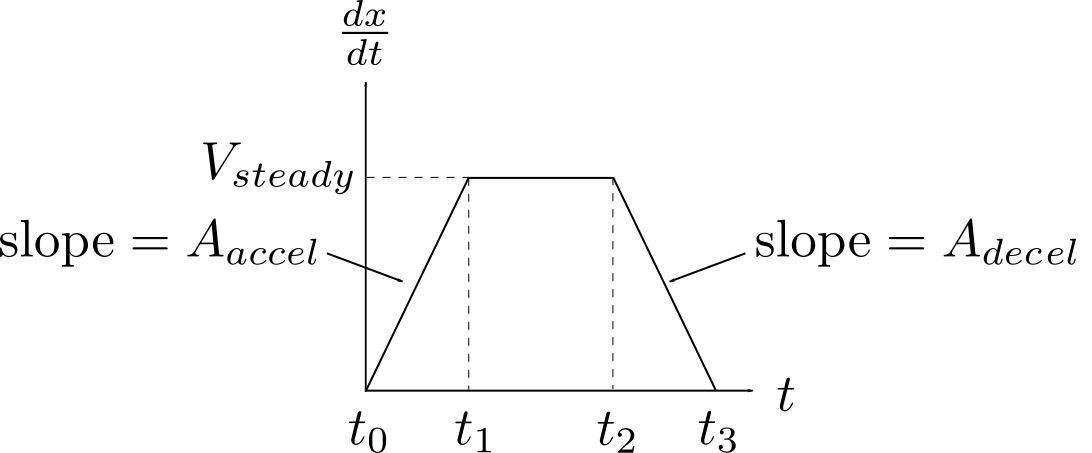
\includegraphics[width=\textwidth]{velocity_vs_time.png}
        \caption{Velocity vs. Time}
        \label{fig:velocity_vs_time}
    \end{subfigure}
    \caption{The trapezoid-shaped trajectory.}
    \label{fig:trapezoid_trajectory}
\end{figure}

 \noindent As shown in Figure~\ref{fig:trapezoid_trajectory}, the initial position is $X_{init}$ and the final position is $X_{final}$. The initial acceleration is $A_{accel}$ and the final deceleration is $A_{decel}$. The maximum velocity is upper bounded by $V_{steady}$. Currently the initial and final velocities are assumed to be zero. Overall, the trajectory is split into three phases:

\begin{enumerate}
\item A constant acceleration phase from time $t_0$ to $t_1$
\item A constant velocity phase from time $t_1$ to $t_2$
\item A constant deceleration phase from time $t_2$ to $t_3$
\end{enumerate}

\noindent The inputs to the trajectory generation algorithm are shown in Table~\ref{table:inputs}.

\begin{table}[tbh]
  \centering
  \begin{tabular}{|l|l|}
   \hline
    \textbf{Variable}                  & \textbf{Description} \\
    \hline
    $X_{init}$         & initial position \\
    $X_{final}$      & final position \\
    $V_{steady}$  & the steady-state (i.e., maximum) velocity \\
    $A_{accel}$     & the initial acceleration \\
    $A_{decel}$  & the final deceleration \\
  \hline
  \end{tabular}
  \vspace{1mm}
  \caption{The input variables to the trajectory generator.}
  \label{table:inputs}
\end{table}

\section{Derivation of Trajectory}

\subsection{Time Accelerating and Decelerating}

Let $T_{accel}$ be the time spent accelerating and $T_{decel}$ be the time spent decelerating. Assuming the maximum velocity is reached, they are defined as:

\begin{equation}
T_{accel} = \abs{V_{steady} / A_{accel}} \label{eq:time_accel_to_max_vel}
\end{equation}

\begin{equation}
T_{decel} = \abs{V_{steady} / A_{decel}} \label{eq:time_dec_from_max_vel}
\end{equation}

Since the accelerations are constant, the distance traveled is equal to the time spent accelerating multiplied by half of the velocity. Thus, the total distance covered accelerating and decelerating is:

\begin{equation}
D_{accel} = (T_{accel} +  T_{decel}) \cdot \frac{|V_{steady}|}{2}
\end{equation}

There are two cases. The first case is if $D_{accel} \le |X_{final} - X_{init}|$, the trajectory will reach $V_{steady}$. This case will be handled in Section~\ref{sec:able_to_reach_V_steady}. The second case is if $D_{accel} > |X_{final} - X_{init}|$, the trajectory will not reach $V_{steady}$. This case will be handled in Section~\ref{sec:unable_to_reach_V_steady}.

\subsection{Case 1: $V_{steady}$ is Reached} \label{sec:able_to_reach_V_steady}

Let $T_{steady}$ be the amount of time spent at $V_{steady}$, i.e., $t_2 - t_1$. The equation for $T_{steady}$ is: 

\begin{equation}
T_{steady} = \frac{|X_{final} - X_{init}| - D_{accel}}{|V_{steady}|}
\end{equation}

\noindent The times $t_0$, $t_1$, $t_2$, and $t_3$, can now be derived:

\begin{eqnarray}
t_0 & = & 0 \\
t_1 & = & T_{accel} \\
t_2 & = & t_1 + T_{steady} \\
t_3 & = & t_2 + T_{decel} 
\end{eqnarray}

\noindent To derive the velocity vs. Time equation, we need to compute the trajectory between times $t_2$ and $t_3$. The equation is given by:

\begin{equation}
\frac{dx}{dt} = A_{decel} \cdot t + c_1 
\label{eq:velocity_vs_time_phase3_1}
\end{equation}

\noindent Variable $c_1$ is where the line intersects the $\frac{dx}{dt}$ axis.  We know that the line must cross the point $t = t_3$ and $\frac{dx}{dt} = 0$. Plugging in these values to equation~\ref{eq:velocity_vs_time_phase3_1}, we get:

\begin{eqnarray}
0 & = & A_{decel} \cdot t_3 + c_1\nonumber \\
c_1 & = & -A_{decel} \cdot t_3
\end{eqnarray}

\noindent Thus, the equation for the velocity vs. time equation is:

\begin{equation}
\frac{dx}{dt}(t) = \left\{
  \begin{array}{rl}
     A_{accel}  \cdot t & \text{if } 0 \le t \le t_1\\
    V_{steady} & \text{if } t_1 \le t \le t_2 \\
     A_{decel}  \cdot t + c_1 & \text{if } t_2 \le t \le t_3 
  \end{array} \right.
\label{eq:case1_velocity_vs_time}
\end{equation}

\noindent We now derive the position vs. time equation by integrating equation~\ref{eq:case1_velocity_vs_time}.

\begin{equation}
x(t) = \left\{
  \begin{array}{rl}
    X_{init} &  \text{if }  t  \le t_0\\
    \frac{A_{accel}}{2} \cdot t^{2} + X_{init} &  \text{if } t_0 \le t \le t_1\\
    V_{steady} \cdot t + c_2 & \text{if } t_1 \le t \le t_2 \text{~and~} t_1 \ne t_2\\
    \frac{A_{decel}}{2} \cdot t^{2} + c_1 \cdot t + c_3 & \text{if } t_2 \le t \le t_3 \\
     X_{final} & \text{if } t \ge t_3 
  \end{array} \right.
 \label{eq:case1_position_vs_time}
\end{equation}

\noindent Constant $c_2$ in equation~\ref{eq:case1_position_vs_time} can be computed by plugging in $t = t_1$ and $x(t_1) = \frac{A_{accel}}{2} \cdot t_1^2 + X_{init}$ as shown below.

\begin{eqnarray}
x(t) & = & V_{steady} \cdot t + c_2 \nonumber \\
 \frac{A_{accel}}{2} \cdot t_1^2 + X_{init} & = & V_{steady} \cdot t_1 + c_2 \nonumber\\
 c_2 & = &   \frac{A_{accel}}{2} \cdot t_1^2 + X_{init} - V_{steady} \cdot t_1
 \end{eqnarray}

\noindent Constant $c_3$ in equation~\ref{eq:case1_position_vs_time} can be computed by plugging in $t = t_2$ and $x(t_2) = V_{steady} \cdot t_2 + c_2$ as shown below.

\begin{eqnarray}
x(t) & = & \frac{A_{decel}}{2} \cdot t^{2} + c_1 \cdot t + c_3 \nonumber \\
V_{steady} \cdot t_2 + c_2 & = & \frac{A_{decel}}{2} \cdot t_2^2 + c_1 \cdot t_2 + c_3 \nonumber \\
 c_3 & = & V_{steady} \cdot t_2 + c_2 - \frac{A_{decel}}{2} \cdot t_2^2 - c_1 \cdot t_2 
  \end{eqnarray}

\noindent This concludes the derivation of the position vs. time trajectory for case 1 where $V_{steady}$ is reachable.

\subsection{Case 2: $V_{steady}$ is Not Reached} \label{sec:unable_to_reach_V_steady}.

In this case, the steady state velocity $V_{steady}$ is not reached because the joint does not accelerate and decelerate fast enough given the distance being traveled. The trajectories in this case are shown in Figure~\ref{fig:case2_trajectories}

\begin{figure}[tbh]
    \centering
    \begin{subfigure}[b]{0.35\textwidth}
        \centering
        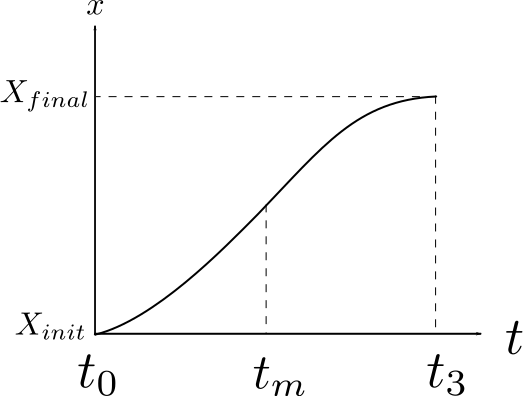
\includegraphics[width=\textwidth]{case2_position_vs_time.png}
        \caption{Position vs. Time plot}
        \label{fig:case2_position_vs_time}
    \end{subfigure}
    \hfill
    \begin{subfigure}[b]{0.525\textwidth}
        \centering
        \includegraphics[width=\textwidth]{case2_velocity_vs_time.png}
        \caption{Velocity vs. Time plot}
        \label{fig:case2_velocity_vs_time}
    \end{subfigure}
    \caption{The trajectory when $V_{steady}$ is not reached.}
    \label{fig:case2_trajectories}
\end{figure}

\noindent There are three unknowns: the maximum velocity reached $V_{max}$, the time between acceleration and deceleration $t_m$, and the total time $t_3$. The equation for the velocity vs. time plot is:

\begin{equation}
\frac{dx}{dt}(t) = \left\{
  \begin{array}{rl}
     A_{accel}  \cdot t & \text{if } 0 \le t \le t_m\\
     A_{decel}  \cdot t + c_4 & \text{if } t_m \le t \le t_3 
  \end{array} \right.
\label{eq:case2_velocity_vs_time}
\end{equation}

\noindent the equation for the position vs. time plot is:

\begin{equation}
x(t)  = \left\{
  \begin{array}{rl}
     \frac{A_{accel}}{2}  \cdot t^2 + X_{init} & \text{if } 0 \le t \le t_m\\
    \frac{A_{decel}}{2}  \cdot t^2 + c_4 \cdot t + c_5 & \text{if } t_m \le t \le t_3 
  \end{array} \right.
\label{eq:case2_position_vs_time}
\end{equation}

\noindent We now derive the values for $t_3$, $t_m$, $c_4$, and $c_5$. Plug $\frac{dx}{dt}(t_3) = 0$ into the second portion of equation~\ref{eq:case2_velocity_vs_time}:

\begin{eqnarray}
\frac{dx}{dt}(t_3) & = &  A_{decel} \cdot t_3 + c_4 \nonumber \\
0 & = &  A_{decel} \cdot t_3 + c_4 \nonumber \\
c_4 & = & -A_{decel} \cdot t_3 \label{eq:case2_c4_in_terms_of_t3}
\end{eqnarray}

\noindent At time $t = t_m$, the two parts of Equation~\ref{eq:case2_velocity_vs_time} are both equal to $V_{max}$. Set them equal and solve for $c_4$:

\begin{eqnarray}
A_{accel} \cdot t_m & = & A_{decel} \cdot t_m + c_4 \nonumber \\
c_4 & = & A_{accel} \cdot t_m - A_{decel} \cdot t_m \nonumber \\
c_4 & = & (A_{accel} - A_{decel}) \cdot t_m \label{eq:case2_c4_in_terms_of_tm}
\end{eqnarray}

\noindent Since Equations~\ref{eq:case2_c4_in_terms_of_t3} and~\ref{eq:case2_c4_in_terms_of_tm} are both for $c_4$, we can set them equal to each other and solve for $t_3$ in terms of $t_m$:

\begin{eqnarray}
-A_{decel} \cdot t_3 & = & (A_{accel} - A_{decel}) \cdot t_m \nonumber \\
t_3 & = & \frac{A_{accel} - A_{decel}}{-A_{decel}} \cdot t_m \nonumber \\
t_3 & = & \frac{A_{decel} - A_{accel}}{A_{decel}} \cdot t_m \label{eq:case2_t3_in_terms_of_tm}
\end{eqnarray}

\noindent At $t=t_m$, both parts of Equation~\ref{eq:case2_position_vs_time} are equal. Let $t=t_m$. Set both sides of Equation~\ref{eq:case2_position_vs_time} to be equal to each other and then solve for zero:

\begin{eqnarray}
\frac{A_{accel}}{2}  \cdot t_m^2 + X_{init} & = & \frac{A_{decel}}{2}  \cdot t_m^2 + c_4 \cdot t_m + c_5 \nonumber \\
0 & = & \left( \frac{A_{decel} - A_{accel}}{2} \right)  \cdot t_m^2 + c_4 \cdot t_m + c_5 - X_{init} \label{eq:case2_time_tm_position}
\end{eqnarray}

\noindent Plug Equation~\ref{eq:case2_c4_in_terms_of_tm} into Equation~\ref{eq:case2_time_tm_position}  to eliminate $c_4$:

\begin{eqnarray}
0  & = & \left( \frac{A_{decel} - A_{accel}}{2} \right)  \cdot t_m^2 + (A_{accel} - A_{decel}) \cdot t^2_m + c_5 - X_{init} \nonumber \\
0 & = &  \left( \frac{A_{accel} - A_{decel}}{2} \right)  \cdot t_m^2 + c_5 - X_{init} \label{eq:case2_time_tm_position2}
\end{eqnarray}

\noindent At time $t=t_3$, $x(t_3) = X_{final}$. Plug these values into the second portion of Equation~\ref{eq:case2_position_vs_time} and solve for zero:

\begin{eqnarray}
X_{final} & = & \frac{A_{decel}}{2}  \cdot t_3^2 + c_4 \cdot t_3 + c_5 \nonumber \\
0 & = &  \frac{A_{decel}}{2}  \cdot t_3^2 + c_4 \cdot t_3 + c_5 - X_{final} \label{eq:case2_time_t3_position}
\end{eqnarray}

\noindent Plug Equation~\ref{eq:case2_c4_in_terms_of_t3} into Equation~\ref{eq:case2_time_t3_position} to elimate $c_4$:

\begin{eqnarray}
0 & = &  \frac{A_{decel}}{2}  \cdot t_3^2 + (-A_{decel}) \cdot t^2_3 + c_5 - X_{final} \nonumber \\
0 & = &  \frac{-A_{decel}}{2}  \cdot t_3^2 + c_5 - X_{final} \label{eq:case2_time_t3_position2}
\end{eqnarray}

\noindent Set Equation~\ref{eq:case2_time_tm_position2} equal to Equation~\ref{eq:case2_time_t3_position2} and simplify:

\begin{eqnarray}
 \left( \frac{A_{accel} - A_{decel}}{2} \right)  \cdot t_m^2 + c_5 - X_{init} & = &  \frac{-A_{decel}}{2}  \cdot t_3^2 + c_5 - X_{final} \nonumber \\
 \left( \frac{A_{accel} - A_{decel}}{2} \right)  \cdot t_m^2 - X_{init} & = &  \frac{-A_{decel}}{2}  \cdot t_3^2 - X_{final} \nonumber\\
\left( \frac{A_{accel} - A_{decel}}{2} \right)  \cdot t_m^2  + \frac{A_{decel}}{2}  \cdot t_3^2 & = &  X_{init} - X_{final}  \label{eq:case2_reduction1}
\end{eqnarray}

\noindent To eliminate $t_3$, plug Equation~\ref{eq:case2_t3_in_terms_of_tm} into Equation~\ref{eq:case2_reduction1}.

\begin{eqnarray}
\left( \frac{A_{accel} - A_{decel}}{2} \right)  \cdot t_m^2  + \frac{A_{decel}}{2}  \cdot \left(\frac{A_{decel} - A_{accel}}{A_{decel}} \cdot t_m\right)^2 & = &  X_{init} - X_{final} \nonumber \\
\left( \frac{A_{accel} - A_{decel}}{2} \right)  \cdot t_m^2  + \frac{A_{decel}}{2}  \cdot \frac{(A_{decel} - A_{accel})^2}{A^2_{decel}} \cdot t^2_m & = &  X_{init} - X_{final}  \nonumber\\
\left( \frac{A_{accel} - A_{decel}}{2} \right)  \cdot t_m^2  +  \frac{(A_{decel} - A_{accel})^2}{2 \cdot A_{decel}} \cdot t^2_m & = &  X_{init} - X_{final} \nonumber \\
\left( \frac{A_{decel} \cdot (A_{accel} - A_{decel}) + (A_{decel} - A_{accel})^2}{2 \cdot A_{decel}} \right)  \cdot t_m^2  & = &  X_{init} - X_{final}  \nonumber\\
\left( \frac{A_{decel} \cdot (A_{accel} - A_{decel}) + (A_{accel} - A_{decel})^2}{2 \cdot A_{decel}} \right)  \cdot t_m^2  & = &  X_{init} - X_{final}  \nonumber\\
\left( \frac{(A_{decel} + A_{accel} - A_{decel}) \cdot (A_{accel} - A_{decel})}{2 \cdot A_{decel}} \right)  \cdot t_m^2  & = &  X_{init} - X_{final} \nonumber \\
\left( \frac{A_{accel} \cdot (A_{accel} - A_{decel})}{2 \cdot A_{decel}} \right)  \cdot t_m^2  & = &  X_{init} - X_{final} \label{eq:case2_reduction2}
\end{eqnarray}

\noindent Solve Equation~\ref{eq:case2_reduction2} for $t_m$:

\begin{eqnarray}
A_{accel} \cdot (A_{accel} - A_{decel})  \cdot t_m^2  & = &  2 \cdot A_{decel} \cdot (X_{init} - X_{final}) \nonumber \\
t_m^2  & = &  \frac{2 \cdot A_{decel} \cdot (X_{init} - X_{final})}{A_{accel} \cdot (A_{accel} - A_{decel})} \nonumber \\
t_m  & = & \sqrt{\frac{2 \cdot A_{decel} \cdot (X_{init} - X_{final})}{A_{accel} \cdot (A_{accel} - A_{decel})}} \label{eq:case2_reduction3}
\end{eqnarray}


%
%
%
%
%
%\noindent To replace $t_3$ with $t_m$ in Equation~\ref{eq:case2_time_t3_position}, plug Equation~\ref{eq:case2_t3_in_terms_of_tm} into Equation~\ref{eq:case2_time_t3_position}.
%
%\begin{eqnarray}
%0 & = &  \frac{A_{decel}}{2}  \cdot \left( \frac{A_{decel} - A_{accel}}{A_{decel}} \cdot t_m \right)^2 + c_4 \cdot \frac{A_{decel} - A_{accel}}{A_{decel}} \cdot t_m  \label{eq:case2_time_t3_position_in_terms_of_tm} \\
% & & + c_5 - X_{final} \nonumber
%\end{eqnarray}
%
%\noindent Set Equations~\ref{eq:case2_time_tm_position} and~\ref{eq:case2_time_t3_position_in_terms_of_tm} to be equal.
%
%\begin{dmath}
%\left( \frac{A_{decel} - A_{accel}}{2} \right)  \cdot t_m^2 + c_4 \cdot t_m + c_5 - X_{init}  = \\
% \frac{A_{decel}}{2}  \cdot \left( \frac{A_{decel} - A_{accel}}{A_{decel}} \cdot t_m \right)^2  + c_4 \cdot\frac{A_{decel} - A_{accel}}{A_{decel}} \cdot t_m + c_5 - X_{final}
%\label{eq:case2_reduction1} 
%\end{dmath}
%
%%\begin{eqnarray}
%%\left( \frac{A_{decel}}{2} - \frac{A_{accel}}{2} \right)  \cdot t_m^2 & = &  \frac{A_{decel}}{2}  \cdot \left( \frac{A_{decel} - A_{accel}}{A_{decel}} \cdot t_m \right)^2   \label{eq:case2_reduction1} \\
%%+ c_4 \cdot t_m + c_5 - X_{init} & & + c_4 \cdot\frac{A_{decel} - A_{accel}}{A_{decel}} \cdot t_m + c_5 - X_{final} \nonumber
%%\end{eqnarray}
%
%\noindent We can solve Equation~\ref{eq:case2_reduction1} for zero and gather like terms:
%
%\begin{dmath}
%\left( \frac{A_{decel} - A_{accel}}{2} - \frac{A_{decel}}{2} \cdot \left(\frac{A_{decel} - A_{accel}}{2}\right)^2\right) \cdot t^2_m + \left(c_4 - c_4 \cdot \frac{A_{decel} - A_{accel}}{A_{decel}} \right) \cdot t_m + X_{final} - X_{init}  = 0
%\label{eq:case2_reduction2} 
%\end{dmath}
%
%\noindent Equation~\ref{eq:case2_reduction2} contains two variables: $c_4$ and $t_m$. To replace $c_4$ with $t_m$ in Equation~\ref{eq:case2_reduction2}, plug Equation~\ref{eq:case2_c4_in_terms_of_tm} into ~\ref{eq:case2_reduction2}:
%
%\begin{dmath}
%\left( \frac{A_{decel} - A_{accel}}{2} - \frac{A_{decel}}{2} \cdot \left(\frac{A_{decel} - A_{accel}}{2}\right)^2\right) \cdot t^2_m + \left( (A_{accel} - A_{decel}) \cdot t_m -  (A_{accel} - A_{decel}) \cdot t_m \cdot \frac{A_{decel} - A_{accel}}{A_{decel}} \right) \cdot t_m + X_{final} - X_{init}  = 0
%\label{eq:case2_reduction3} 
%\end{dmath}
%
%\noindent We can combine the $t_m$ variables in the middle of Equation~\ref{eq:case2_reduction3} as follows:
%
%\begin{dmath}
%\left( \frac{A_{decel} - A_{accel}}{2} - \frac{A_{decel}}{2} \cdot \left(\frac{A_{decel} - A_{accel}}{2}\right)^2\right) \cdot t^2_m + \left( (A_{accel} - A_{decel}) -  (A_{accel} - A_{decel}) \cdot \frac{A_{decel} - A_{accel}}{A_{decel}} \right) \cdot t^2_m + X_{final} - X_{init}  = 0
%\label{eq:case2_reduction4} 
%\end{dmath}
%
%\noindent The two intances of $t^2_m$ in Equation~\ref{eq:case2_reduction4} can be combined:
%
%\begin{dmath}
%\left( \frac{A_{decel} - A_{accel}}{2} - \frac{A_{decel}}{2} \cdot \left(\frac{A_{decel} - A_{accel}}{2}\right)^2 + (A_{accel} - A_{decel}) -  (A_{accel} - A_{decel}) \cdot \frac{A_{decel} - A_{accel}}{A_{decel}} \right) \cdot t^2_m + X_{final} - X_{init}  = 0
%\label{eq:case2_reduction5} 
%\end{dmath}
%
%\noindent Now we can solve for $t_m$:
%
%\begin{dmath}
%t_m = \sqrt{\frac{X_{init} - X_{final}}{c_6}}
%\label{eq:case2_tm}
%\end{dmath}
%
%\noindent where:
%
%\begin{dmath}
%c_6 = \frac{A_{decel} - A_{accel}}{2} - \frac{A_{decel}}{2} \cdot \left(\frac{A_{decel} - A_{accel}}{2}\right)^2 + (A_{accel} - A_{decel}) -  (A_{accel} - A_{decel}) \cdot \frac{A_{decel} - A_{accel}}{A_{decel}}
%\end{dmath}

\noindent The rest of the unknowns can now be easily computed:

\begin{itemize}
\item To compute $c_4$, plug $t_m$ into Equation~\ref{eq:case2_c4_in_terms_of_tm}.
\item To compute $t_3$, plug $c_4$ into Equation~\ref{eq:case2_c4_in_terms_of_t3}.

\begin{equation}
t_3 = \frac{c_4}{-1 \cdot A_{decel}}
\end{equation}

\item To compute $c_5$, plug $t_3$ and $c_4$ into Equation~\ref{eq:case2_time_t3_position}.
\begin{equation}
c_5 = X_{final} - c_4 \cdot t_3 - \frac{A_{decel}}{2} \cdot t_3^2
\end{equation}

\end{itemize}

\noindent Comparing equation~\ref{eq:case1_velocity_vs_time} with~\ref{eq:case2_velocity_vs_time} and equation~\ref{eq:case1_position_vs_time} with~\ref{eq:case2_position_vs_time}, we can see that the same position vs. time and velocity vs. time equations can be used in both cases. Specifically, case 2 can use case 1 equations by setting:

\begin{eqnarray}
c_1 & = & c_4\\
c_3 & = & c_5\\
t_1  & = & t_m\\
t_2 & = & t_m
\end{eqnarray}

\noindent This concludes the derivation of the trapezoid velocity-shaped trajectory.
\end{document}
